\section{Auswertung}
Die in der Auswertung bestimmten Ausgleichsrechnungen werden mit
dem Python Paket \emph{scipy.optimize}\cite{scipy} durchgeführt.
Des Weiteren werden die Fehler und insbesondere die Fehlerfortpflanzungen
mit dem Python Paket \emph{uncertainties}\cite{uncertainties} berechnet.

\subsection{Regressionsberechnung zur Bestimmung der Spannung im Verhältnis zum Abstand}

Für die verschiedenen Auswertungsteile wird immer eine Umrechnung von gemessenen Abständen
in die Spannung $U$ benötigt. Dazu wird an die Messwerte die in den Tabellen \ref{}- \ref{} dargestellt sind,
eine Gerade der Form
\begin{equation*}
  g(x)=mx+b
\end{equation*}
berechnet.
\begin{table} 
\centering 
\caption{Aus Abbildung \ref{} abgelesene Spannung-Abstandspaare.} 
\label{tab: spannung_abstand_zim} 
\begin{tabular}{S S } 
\toprule  
{Abstand in $\si{\centi\meter}$} & {Spannung in $\si{\volt}$}  \\ 
\midrule  
 2.0  & 1.0\\ 
4.0  & 2.0\\ 
6.1  & 3.0\\ 
8.2  & 4.0\\ 
10.3  & 5.0\\ 
12.5  & 6.0\\ 
14.6  & 7.0\\ 
16.7  & 8.0\\ 
18.8  & 9.0\\ 
21.3  & 10.0\\ 
\bottomrule 
\end{tabular} 
\end{table}
\begin{table} 
\centering 
\caption{Aus Abbildung \ref{fig: messkurve_energie_hot} abgelesene Spannung-Abstandspaare.} 
\label{tab: spannung_abstand_hot} 
\begin{tabular}{S S } 
\toprule  
{Abstand in $\si{\centi\meter}$} & {Spannung in $\si{\volt}$}  \\ 
\midrule  
 1.9  & 1\\ 
4.1  & 2\\ 
6.1  & 3\\ 
8.3  & 4\\ 
10.2  & 5\\ 
12.3  & 6\\ 
14.5  & 7\\ 
16.7  & 8\\ 
18.8  & 9\\ 
20.9  & 10\\ 
\bottomrule 
\end{tabular} 
\end{table}
\begin{table} 
\centering 
\caption{Aus Abbildung \ref{fig: messkurve_frank_hertz} abgelesene Spannung-Abstandspare.} 
\label{tab: spannung_abstand_frank} 
\begin{tabular}{S S } 
\toprule  
{Abstand in $\si{\centi\meter}$} & {Spannung in $\si{\volt}$}  \\ 
\midrule  
 2.1  & 5\\ 
4.0  & 10\\ 
6.0  & 15\\ 
7.9  & 20\\ 
9.8  & 25\\ 
11.8  & 30\\ 
13.8  & 35\\ 
15.8  & 40\\ 
19.7  & 50\\ 
21.7  & 55\\ 
\bottomrule 
\end{tabular} 
\end{table}
\begin{table} 
\centering 
\caption{Aus Abbildung \ref{fig: messkurve_ioni} abgelesene Punkte, durch die eine Ausgleichgerade gelegt wird.} 
\label{tab: kodi_ioni} 
\begin{tabular}{S S } 
\toprule  
{Abstand in $\si{\centi\meter}$} & {Spannung in $\si{\volt}$}  \\ 
\midrule  
 1.3  & 2\\ 
2.7  & 4\\ 
4.2  & 6\\ 
5.4  & 8\\ 
6.8  & 10\\ 
8.0  & 12\\ 
9.4  & 14\\ 
10.5  & 16\\ 
12.0  & 18\\ 
13.5  & 20\\ 
14.5  & 22\\ 
15.8  & 24\\ 
17.2  & 26\\ 
18.5  & 28\\ 
\bottomrule 
\end{tabular} 
\end{table}
Die sich daraus ergebenenen Regressionparameter sind in Tabelle \ref{tab: umrech} aufgelistet.
\begin{table} 
\centering 
\caption{Regressiongerade für die Abstand in Spannungs Umrechnung. Im Versuchsteil $1$ wird die Energieverteilung bei $T=\SI{28}{\celsius}$ untersucht, $2$ umfassst die Untersuchung der Energieverteilung bei $T=\SI{155}{\celsius}$, der dritte Abschnitt $(3)$ beschäftigt sich mit der Analyse der Frank-Hertz-Kurve und im Abschnitt $4$ wird die Ionisierungsspannung bestimmt.} 
\label{tab: umrech} 
\begin{tabular}{S S S S S } 
\toprule  
{Versuchsteil} & { $m$ in $\si{\volt\centi\meter\per}$} & {$\sigma_\mathrm{m}$ in $\si{\volt\centi\per\meter}$} & {$b$ in $\si{\volt}$} & {$\sigma_\mathrm{b}$ in $\si{\volt}$}  \\ 
\midrule  
 1  & 0.469  & 0.003  & 0.13  & 0.04\\ 
2  & 0.475  & 0.002  & 0.13  & 0.03\\ 
3  & 2.549  & 0.006  & -0.20  & 0.08\\ 
4  & 1.522  & 0.009  & -0.19  & 0.10\\ 
\bottomrule 
\end{tabular} 
\end{table}

Die Messwerte aus den Tabellen \ref{}- \ref{} und die dazugehörigen Ausgleichsgeraden sind in
den Abbildungen \ref{} und \ref{} illustriert.
\begin{figure}
  \centering
  \begin{subfigure}{0.48\textwidth}
    \centering
    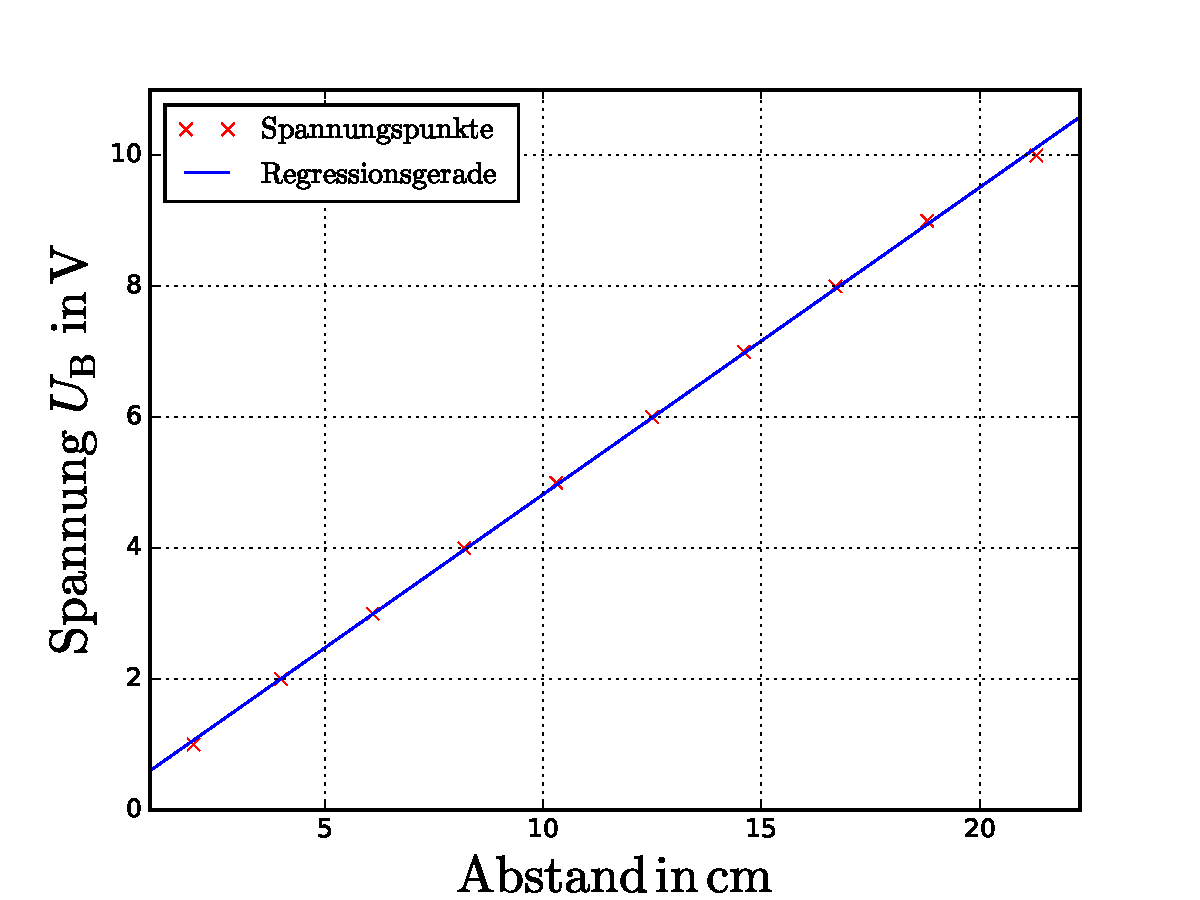
\includegraphics[width=1 \textwidth]{../Messdaten/zim.pdf}
    \caption{Graphische Darstellung des Ausgleichgraden für die Energieverteilung bei $\SI{28}{\degree}$.}
    \label{fig: energie_zim}
  \end{subfigure}
  \begin{subfigure}{0.48\textwidth}
    \centering
    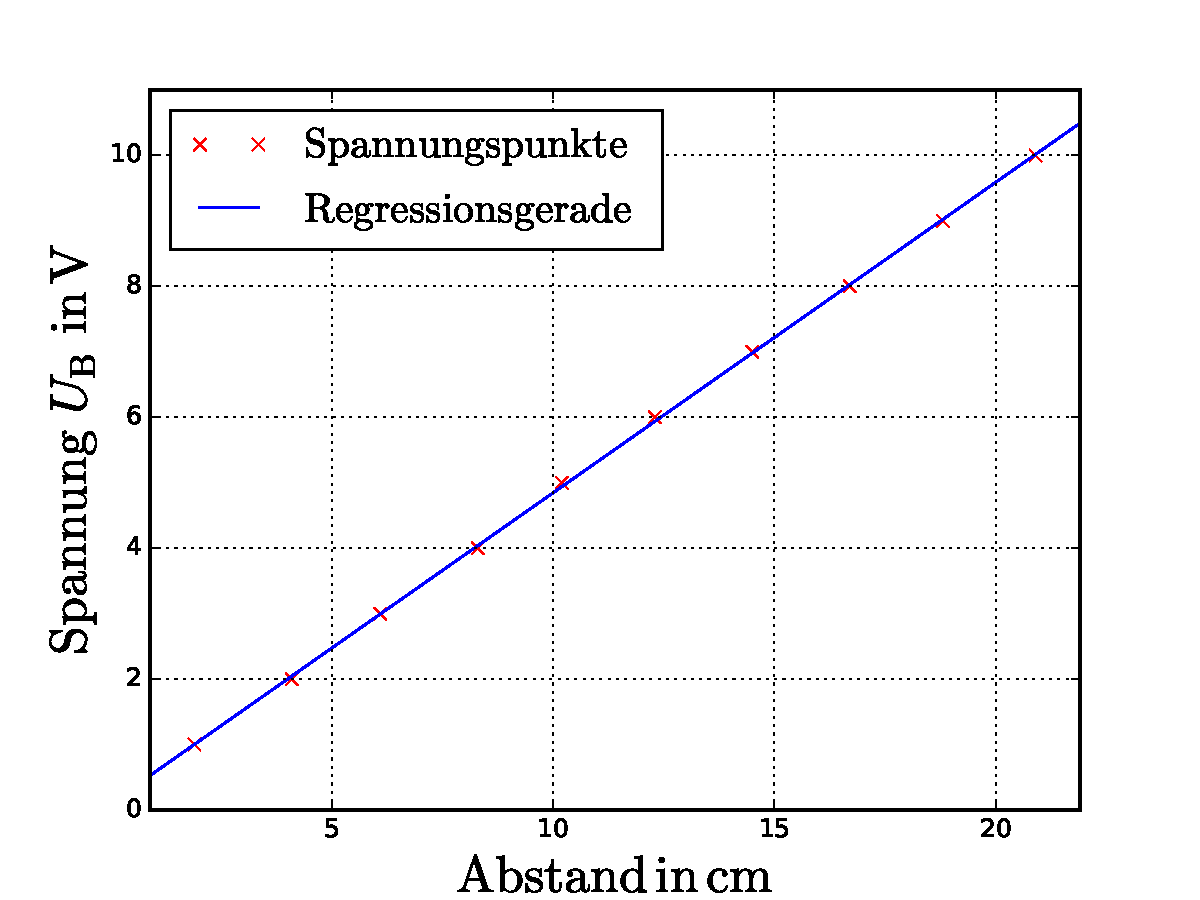
\includegraphics[width=1 \textwidth]{../Messdaten/spannungsfit_energieverteilung_150grad.pdf}
    \caption{Graphische Darstellung des Ausgleichgraden für die Energieverteilung bei $\SI{155}{\degree}$.}
    \label{fig: enrgie_hot}
  \end{subfigure}
  \caption{Darstellung der Ausgleichsgeraden für $(1)$ und $(2)$}
  \label{fig: darstellung_1}
\end{figure}

\begin{figure}
  \centering
  \begin{subfigure}{0.48\textwidth}
    \centering
    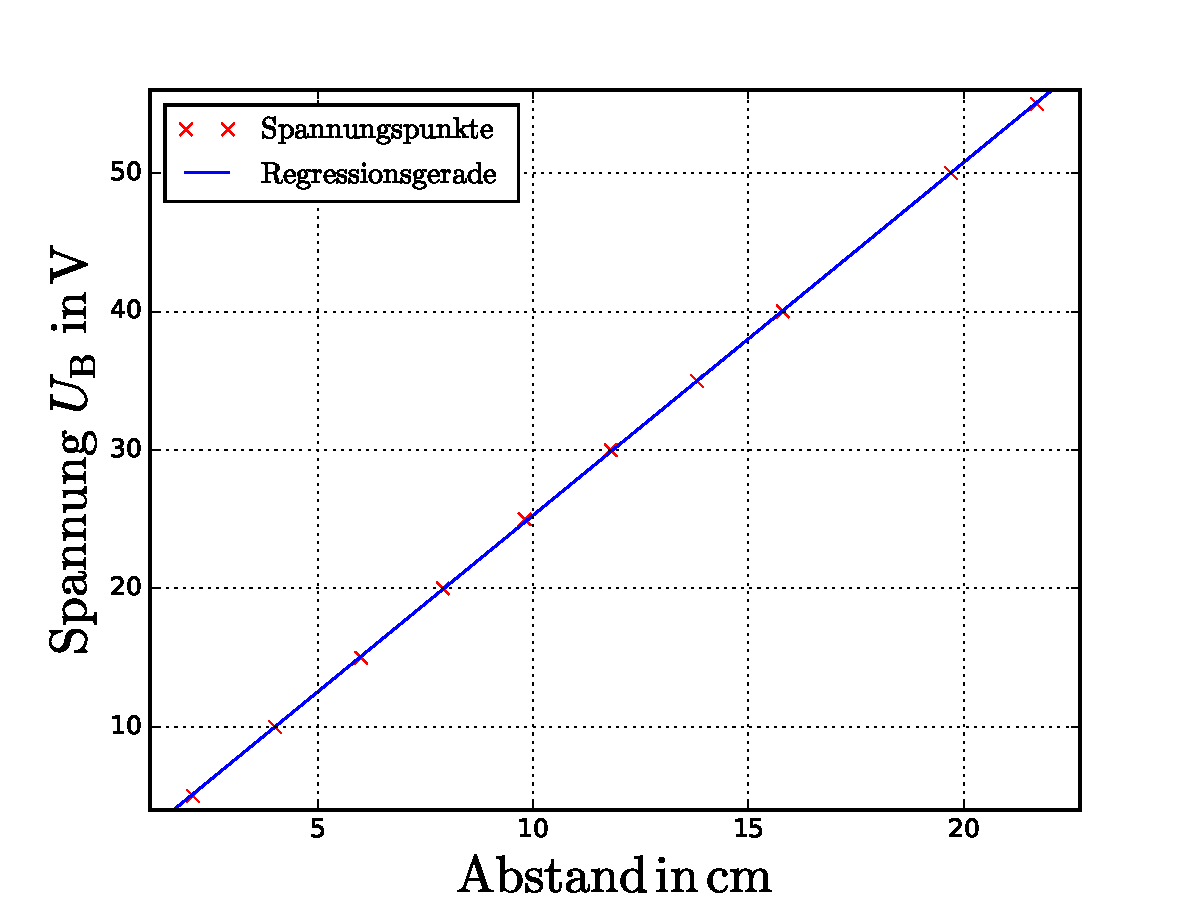
\includegraphics[width=1 \textwidth]{../Messdaten/frank_hertz_kuvre.pdf}
    \caption{Graphische Darstellung des Ausgleichgraden für Frank-Hertz-Kurve.}
    \label{fig: frank_hertz}
  \end{subfigure}
  \begin{subfigure}{0.48\textwidth}
    \centering
    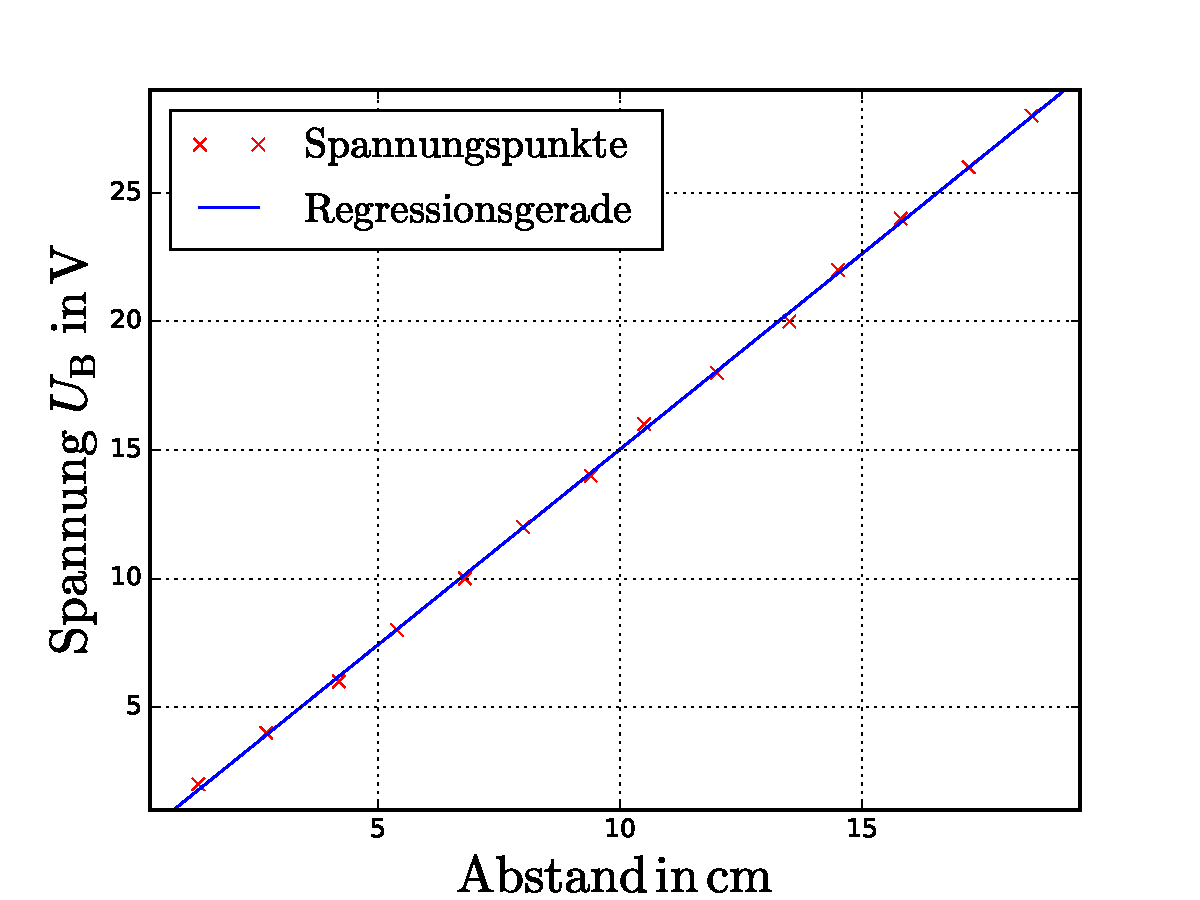
\includegraphics[width=1 \textwidth]{../Messdaten/ioni.pdf}
    \caption{Graphische Darstellung des Ausgleichgraden für die Untrersuchung der Ionisierungsspannung.}
    \label{fig: enrgie_hot}
  \end{subfigure}
  \caption{Darstellung der Ausgleichsgeraden für $(3)$ und $(4)$}
  \label{fig: darstellung_2}
\end{figure}
